
\subsection{Especificación de casos de uso}

Este documento contiene la descripción de los casos de uso. El modelo 
de casos de uso es un modelo de las funciones que realiza el sistema y 
su entorno, y sirve de contrato entre el cliente y los desarrolladores. 
Se emplea como entrada para las actividades de análisis, diseño y test.

Este documento contiene además aquellos requisitos que no pueden ser 
obtenidos tan solo con un análisis basado en casos de uso, como los 
requisitos de rendimiento o fiabilidad.

\subsubsection{Actores}

Un actor define un conjunto coherente de roles que los usuarios del 
sistema interpretan cuando interactúan con el mismo. Puede ser un 
individuo o un sistema externo.

Se procederá a enumerar los actores que participan en el sistema, 
así como una breve descripción de cada uno de ellos.

\paragraph{Usuario} Representa a la persona que interacturá con la
base del conocimiento generada. No manipulará los datos, sino que los
usará para hacer consultas y/o busquedas.

\paragraph{Administrador} Representa al usuario que se encargue de 
administrar el servicio y la máquina que lo aloje. Su labores principales
serán la de programar actualizaciones y verificar que hayan resultado
satisfactoriamente.

\subsubsection{Límites del sistema}

En la figura siguiente se establecen los límites del sistema, así 
como los principales casos de uso que posteriormente serán refinados 
en siguientes etapas del análisis.

\begin{figure}
 	\centering
	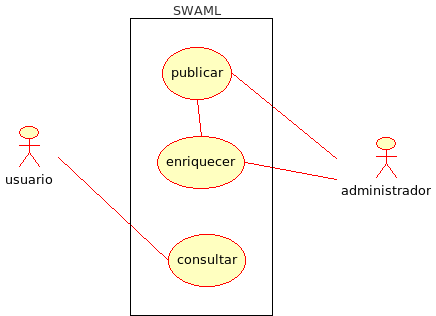
\includegraphics[width=12cm]{images/uml/casos-uso/general.png}
	\caption{Casos generales de uso}
	\label{uml:casos-uso}
\end{figure}

Como se ve en la figura~\ref{uml:casos-uso} se puede disntiguir claramente
tres grandes bloques de casos de uso:

\begin{itemize}
 \item Publicar los datos
 \item Enriquecerlos
 \item Consultarlos
\end{itemize}

\subsubsection{Casos de uso}

Refinando el diagrama anterior se identifican varios casos de uso que paso a
enumerar:

\begin{itemize}
 \item Parametrizar el sistema
 \item Iniciar la publicación
 \item Enriquecer los datos
 \item Consular los archivos generados
 \item Consultar la información extra generada
\end{itemize}


\paragraph{Parametrizar el sistema}

\subparagraph{Descripción}Este caso de uso representa la labor que
el usuario administrador debe realizar para configurar correctamente 
el sistema.

\subparagraph{Flujo de eventos}El caso de uso comienza cuando el
usuario administrador comienza a editar una configuración, bien
manualmente o mediante el asistente que acompaña al software.

\subparagraph{Precondiciones}Es necesario disponer de un mailbox
a exportar.

\subparagraph{Postcondiciones}Ninguna.


\paragraph{Iniciar la publicación}

\subparagraph{Descripción}Representa la acción de publicación propiamente
dicha.

\subparagraph{Flujo de eventos}El proceso es un proceso por lotes que
a partir de una configuración genera una serie de ficheros RDF. Internamente
se divide en varios procesos:
\begin{enumerate}
 \item \emph{Parsear} el mailbox
 \item Revisar la consistencia de todas las relaciones entre los distintos mensajes
 \item Enriquecer la información
 \item Exportar cada uno de estos mensajes en RDF
 \item Exportar los suscriptores en RDF
 \item Exportar los suscriptores en KML si fuese requerido
 \item Exportar todos los indices
\end{enumerate}

\subparagraph{Precondiciones}Disponer de una configuración correcta.

\subparagraph{Postcondiciones}El directorio destino de la exportación
debe poder \emph{consumirse} mediante otro servicio, como un servidor
\texttt{HTTP} (Apache o similar).


\paragraph{Enriquecer los datos}

\subparagraph{Descripción}Representa la interacción del sistema con
otras bases del conocimiento externas, principalmente los FOAF de los
suscriptores a la lista de correo, para enriquecer la información en
determinados aspectos.

\subparagraph{Flujo de eventos}Se tratar de un proceso que se repite
iterativamente con cada uno de los suscriptores:
\begin{enumerate}
 \item Buscar su FOAF
 \item Si lo tiene:
 \begin{enumerate}
  \item	Enlazar al suscriptor con su FOAF
  \item Consultar sus coordenadas geográficas
  \item Consultar su foto
 \end{enumerate}
 \item Si no lo tiene continuar con el siguiente suscriptor
\end{enumerate}


\subparagraph{Precondiciones}Disponer de la lista de suscriptores en
memoria.

\subparagraph{Postcondiciones}Ninguna.


\paragraph{Consular los archivos generados}

\subparagraph{Descripción}Representa la interacción del usuario con los
datos generados. Desde una simple consulta manual a los ficheros RDF
generados, hasta realizar consultas de una forma más sofisticada.

\subparagraph{Flujo de eventos}Consultar, leer, comprender y/o desechar 
la información obtenida.

\subparagraph{Precondiciones}Disponer de la lista exportada a RDF.

\subparagraph{Postcondiciones}Ninguna concreta.


\paragraph{Consultar la información extra generada}

\subparagraph{Descripción}Este caso de uso representa la consulta por
parte del usuario de la información extra generada, por el ejemplo los
suscriptores en formato KML.

\subparagraph{Flujo de eventos}Consultar y explotar.

\subparagraph{Precondiciones}Disponer de la información geográfica de
los suscriptores.

\subparagraph{Postcondiciones}Explotación de estos datos, por ejemplo
visualizandolos\footnote{\url{http://maps.google.es/maps?q=http://swaml.berlios.de/demo/subscribers.kml}} 
con Google Maps\footnote{\url{http://maps.google.es/}}.


